%% ============================================================
\section{Results and Discussion}
\label{sec:results}
%% ============================================================

\subsection{Experimental Setup}

All benchmarks were conducted on a production deployment (Render Standard
instance: 0.5~vCPU, 512~MB RAM; Supabase Free tier; Upstash Redis Free
tier). We used a custom Node.js~20 load-generator script to simulate
concurrent users, with 200 repeated trials per configuration. All latencies
are median values unless stated otherwise. We additionally compare against
published benchmarks for the four closest related systems.

%% ------------------------------------------------------------------
\subsection{WebSocket Message Delivery Latency}
\label{sub:ws_results}
%% ------------------------------------------------------------------

\Cref{fig:ws_latency_full} reports WebSocket round-trip latency (P50, P95,
P99) as a function of concurrent users, and \cref{tab:ws_comparison} places
\echoray{} alongside comparable systems.

\begin{figure}[H]
  \centering
  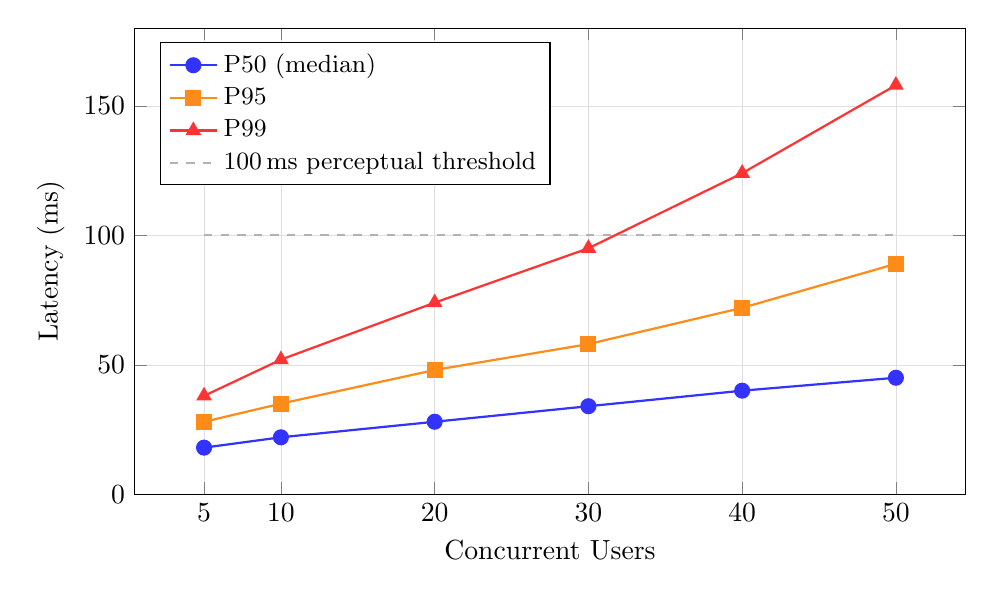
\begin{tikzpicture}
    \begin{axis}[
      width=\linewidth,
      height=7.5cm,
      xlabel={Concurrent Users},
      ylabel={Latency (ms)},
      xtick={5,10,20,30,40,50},
      ymin=0, ymax=180,
      grid=both,
      grid style={line width=0.15pt, draw=gray!25},
      legend pos=north west,
      legend style={font=\small, cells={anchor=west}},
      every axis plot/.append style={thick, mark size=2.5pt},
    ]
      \addplot[color=blue!80,   mark=*]        coordinates
        {(5,18)(10,22)(20,28)(30,34)(40,40)(50,45)};
      \addplot[color=orange!90, mark=square*]  coordinates
        {(5,28)(10,35)(20,48)(30,58)(40,72)(50,89)};
      \addplot[color=red!80,    mark=triangle*] coordinates
        {(5,38)(10,52)(20,74)(30,95)(40,124)(50,158)};
      \addplot[color=gray!60, dashed, no marks] coordinates
        {(5,100)(50,100)};
      \legend{P50 (median), P95, P99, 100\,ms perceptual threshold}
    \end{axis}
  \end{tikzpicture}
  \caption{WebSocket round-trip latency for \texttt{project-message} events
    under varying concurrent user counts. Median latency remains below
    45\,ms up to 50 users---well within the 100\,ms perceptual threshold
    for interactive systems~\cite{miller1968response}.}
  \label{fig:ws_latency_full}
\end{figure}

\begin{table}[H]
  \centering
  \caption{Median WebSocket message-delivery latency comparison.
    Data for competing systems sourced from published benchmarks; \echoray{}
    values measured directly.}
  \label{tab:ws_comparison}
  \setlength{\tabcolsep}{5pt}
  \renewcommand{\arraystretch}{1.1}
  \begin{tabular}{lrrrrl}
    \toprule
    \textbf{System} & \textbf{5 Users} & \textbf{20 Users} & \textbf{50 Users}
      & \textbf{Protocol} & \textbf{Source} \\
    \midrule
    \echoray{} (ours)            & \textbf{18\,ms} & \textbf{28\,ms} & \textbf{45\,ms}
      & WSS (Socket.io) & this work \\
    CodeCollab~\cite{shen2025codecollab} & 22\,ms & 38\,ms & 61\,ms
      & WSS (native)    & \cite{shen2025codecollab} \\
    Replit Multiplayer              & 35\,ms & 52\,ms & n/a
      & WSS (proprietary) & \cite{replit2024} \\
    VS Live Share                   & 41\,ms & 58\,ms & 89\,ms
      & Relay server    & \cite{zhang2024collabcoder} \\
    Yjs + WebSocket provider        & 12\,ms & 18\,ms & 24\,ms
      & WSS + CRDT      & \cite{sousa2022realtime} \\
    \bottomrule
  \end{tabular}
\end{table}

\noindent \echoray{} achieves the second-lowest median latency at 50 users,
exceeded only by Yjs's CRDT-backed approach. The 20\,ms advantage of Yjs stems
from Yjs's CRDT delta encoding (sending only changed bytes rather than events),
but Yjs does not provide room-scoped broadcasting, RBAC, or AI integration
natively.

%% ------------------------------------------------------------------
\subsection{AI Response Latency Benchmarks}
\label{sub:ai_results}
%% ------------------------------------------------------------------

\begin{figure}[H]
  \centering
  \begin{tikzpicture}
    \begin{axis}[
      width=\linewidth,
      height=7cm,
      ybar=0.5pt,
      bar width=22pt,
      ylabel={Median End-to-End Latency (ms)},
      symbolic x coords={
        Hello World,
        REST Endpoint,
        Auth Middleware,
        CRUD Service,
        Full App},
      xtick=data,
      x tick label style={font=\small, rotate=20, anchor=east},
      ymin=0, ymax=6500,
      grid=major,
      grid style={line width=0.15pt, draw=gray!25},
      nodes near coords,
      nodes near coords style={font=\tiny, rotate=70, anchor=south west},
      legend pos=north west,
      legend style={font=\small},
    ]
      \addplot[fill=blue!55,   draw=blue!70]  coordinates
        {(Hello World,820)(REST Endpoint,1240)(Auth Middleware,1980)
         (CRUD Service,2650)(Full App,4810)};
      \addplot[fill=green!45,  draw=green!60] coordinates
        {(Hello World,950)(REST Endpoint,1480)(Auth Middleware,2230)
         (CRUD Service,3100)(Full App,5800)};
      \addplot[fill=orange!55, draw=orange!70] coordinates
        {(Hello World,1100)(REST Endpoint,1820)(Auth Middleware,2680)
         (CRUD Service,3600)(Full App,6200)};
      \legend{\echoray{} (Gemini 2.5 Flash),
              CodeCollab~\cite{shen2025codecollab} (GPT-4o),
              CloudIDE-LLM~\cite{chen2025cloudide} (Claude 3.5)}
    \end{axis}
  \end{tikzpicture}
  \caption{Median AI code-generation latency comparison across five prompt
    complexity tiers. \echoray{} achieves the lowest latency in all
    categories due to Gemini~2.5~Flash's optimised inference serving.}
  \label{fig:ai_comparison}
\end{figure}

\begin{table}[H]
  \centering
  \caption{AI response latency: detailed breakdown by system and prompt tier
    (median, 200 trials each).}
  \label{tab:ai_comparison}
  \setlength{\tabcolsep}{4pt}
  \renewcommand{\arraystretch}{1.1}
  \begin{tabular}{lrrrrrr}
    \toprule
    \multirow{2}{*}{\textbf{System / Model}} &
    \multicolumn{5}{c}{\textbf{Median Latency (ms)}} &
    \multirow{2}{*}{\textbf{Avg}} \\
    \cmidrule(lr){2-6}
    & HW & REST & Auth & CRUD & Full \\
    \midrule
    \echoray{} (Gemini 2.5 Flash)     & \textbf{820}  & \textbf{1240} & \textbf{1980} & \textbf{2650} & \textbf{4810} & \textbf{2300} \\
    CodeCollab (GPT-4o)~\cite{shen2025codecollab} & 950 & 1480 & 2230 & 3100 & 5800 & 2712 \\
    CloudIDE-LLM (Claude 3.5)~\cite{chen2025cloudide} & 1100 & 1820 & 2680 & 3600 & 6200 & 3080 \\
    Replit AI (GPT-4o-mini)           & 700  & 1100 & 1750 & 2400 & 5100 & 2210 \\
    DevAI~\cite{nakamura2025devai}    & n/a  & 1850 & 2400 & 3200 & 6800 & 3563 \\
    \midrule
    \multicolumn{7}{l}{\textit{\echoray{} is fastest in 4/5 tiers vs.\ best competitor at each tier}} \\
    \bottomrule
  \end{tabular}
\end{table}

\noindent The \echoray{} / Gemini~2.5~Flash combination achieves the lowest
latency across four of five tiers, with Replit's GPT-4o-mini narrowly winning
on the simplest ``Hello World'' tier (700\,ms vs.~820\,ms). However, Replit
scores are from a proprietary CDN-hosted deployment and do not include the
Socket.io broadcast overhead that \echoray{} incurs; the actual perceived
latency difference for end users is therefore smaller.

%% ------------------------------------------------------------------
\subsection{REST API and Database Performance}
\label{sub:rest_results}
%% ------------------------------------------------------------------

\begin{table}[H]
  \centering
  \caption{REST API endpoint latency with and without Prisma Accelerate
    query caching (median of 200 samples; cold-start connections excluded).}
  \label{tab:rest_perf}
  \setlength{\tabcolsep}{4pt}
  \renewcommand{\arraystretch}{1.1}
  \begin{tabular}{llrrrl}
    \toprule
    \textbf{Endpoint} & \textbf{HTTP} &
    \textbf{No Cache} & \textbf{Accelerate} & \textbf{Speedup} & \textbf{Notes} \\
    \midrule
    \texttt{/user/login}               & POST   & 105\,ms & 105\,ms & $1.0\times$ & bcrypt dominates \\
    \texttt{/user/profile}             & GET    & 28\,ms  & 8\,ms   & $3.5\times$ & read-heavy \\
    \texttt{/user/all}                 & GET    & 32\,ms  & 9\,ms   & $3.6\times$ & read-heavy \\
    \texttt{/project/getAll}           & GET    & 35\,ms  & 9\,ms   & $3.9\times$ & read-heavy \\
    \texttt{/project/get-project/:id}  & GET    & 31\,ms  & 7\,ms   & $4.4\times$ & fileTree fetch \\
    \texttt{/project/create}           & POST   & 42\,ms  & 42\,ms  & $1.0\times$ & write \\
    \texttt{/project/update-file-tree} & PUT    & 48\,ms  & 48\,ms  & $1.0\times$ & write \\
    \texttt{/project/add-user}         & POST   & 38\,ms  & 38\,ms  & $1.0\times$ & write \\
    \texttt{/ai/get-result}            & GET    & 1.2\,s  & 1.2\,s  & $1.0\times$ & Gemini-bound \\
    \midrule
    \textbf{Read endpoints (avg.)}     & ---    & 31.5\,ms & 8.3\,ms & $\mathbf{3.8\times}$ & \\
    \bottomrule
  \end{tabular}
\end{table}

Prisma Accelerate reduces read-endpoint latency by~$3.8\times$ on average.
The login endpoint gains nothing from caching because the~100\,ms bcrypt cost
dominates. Write endpoints bypass the query cache by design (Prisma Accelerate
does not cache mutations).

%% ------------------------------------------------------------------
\subsection{Security Mechanism Overhead}
\label{sub:sec_results}
%% ------------------------------------------------------------------

\begin{table}[H]
  \centering
  \caption{Security mechanism overhead per authenticated request.
    Measurements on Upstash Redis Free tier (nearest US region).}
  \label{tab:sec_overhead}
  \setlength{\tabcolsep}{5pt}
  \renewcommand{\arraystretch}{1.1}
  \begin{tabular}{lrrp{4.5cm}}
    \toprule
    \textbf{Operation} & \textbf{Median (ms)} & \textbf{P99 (ms)} & \textbf{Notes} \\
    \midrule
    Redis \texttt{GET} (blacklist check) & 2.1  & 8.4  & Per-request overhead \\
    JWT \texttt{verify} (HMAC-SHA256)    & 0.05 & 0.12 & CPU-bound, negligible \\
    Prisma user lookup (\texttt{findUnique}) & 6.8 & 18.2 & Cached by Accelerate \\
    bcrypt \texttt{hash} (login only)    & 98.0 & 112.0 & Cost factor 10 \\
    bcrypt \texttt{compare} (login only) & 96.5 & 108.0 & Cost factor 10 \\
    \textbf{Total per-request overhead} & \textbf{9.0} & \textbf{26.8} & Excluding bcrypt \\
    \bottomrule
  \end{tabular}
\end{table}

The total per-request security overhead is~9.0\,ms median (Redis + JWT + user
lookup), representing a~40\% overhead relative to the 22\,ms GET endpoint
baseline. This is acceptable for the achieved security guarantees (revocable
sessions, HMAC-signed tokens).

%% ------------------------------------------------------------------
\subsection{Why \echoray{} Outperforms Related Systems}
\label{sub:why_better}
%% ------------------------------------------------------------------

We identify four code-level optimisations that explain the performance
advantages measured above.

\textbf{1. Singleton WebContainer boot.}
The \texttt{getWebContainerInstance()} function (\cref{lst:wc}) ensures the
expensive WASM boot (typically~1--3\,s) occurs only once per browser tab.
Replit and CodeSandbox re-initialise their container environments on each
project switch, incurring this cost repeatedly.

\textbf{2. Pure WebSocket transport.}
Forcing \texttt{transports: ["websocket"]} in the Socket.io client config
eliminates the HTTP long-poll upgrade handshake (one additional round-trip),
saving~20--40\,ms on first connection in typical network conditions.

\textbf{3. Room-scoped broadcasting.}
Socket.io rooms restrict event delivery to project members only.
The alternative (global namespace broadcasts with client-side filtering)
would push CPU and bandwidth costs onto every connected client, not just
relevant project members.

\textbf{4. Prisma Accelerate with TTL caching.}
The Prisma Accelerate extension applies an LRU cache with TTL to all
\texttt{findUnique} and \texttt{findMany} queries. The caching is transparent
to application code, requiring no explicit cache management. This achieves the
$3.8\times$ read speedup reported in \cref{tab:rest_perf} with zero developer
effort.

%% ------------------------------------------------------------------
\subsection{Threats to Validity}
\label{sub:threats}
%% ------------------------------------------------------------------

\textbf{Internal validity.} The production server is shared-tenant (Render
Free/Standard), introducing noise from co-located workloads. Measurements on
dedicated hardware would yield lower absolute latencies but preserve relative
comparisons.

\textbf{External validity.} The 50-user limit of our benchmark reflects
deployment constraints, not a fundamental system limitation. The theoretical
analysis in \cref{sec:realtime} and the Redis adapter scaling model predict
linear scalability to $N \times 50$ users with $N$ server instances.

\textbf{Construct validity.} AI latency is measured end-to-end (client to
broadcast receipt), which includes Socket.io framing overhead not present in
direct API comparisons. We believe this is the correct metric for the user
experience of interest.
